\documentclass{article}
\usepackage[spanish]{babel}
\usepackage{amssymb}
\usepackage{amsmath}
\usepackage{graphicx}

\begin{document}

\section*{Ejercicio 1}
\subsection*{a) Existe un término $t \in \Lambda$ tal que para todo $s \in \Lambda$ se tiene que $t\ s =_\beta s\ t$.}

\textbf{Verdadero.} Tomemos \[
    t = (\lambda x. (\lambda y. y x x))\ (\lambda x. (\lambda y. y x x)).
\]

Así, tenemos que 
\begin{align*}
    t\ s &\rightarrow_\beta (\lambda z. z\ (\lambda x. (\lambda y. y x x))\ (\lambda x. (\lambda y. y x x)))\ s\\
    &\rightarrow_\beta s\ (\lambda x. (\lambda y. y x x))\ (\lambda x. (\lambda y. y x x))\\
    &= s\ t.
\end{align*}

\subsection*{b) Existe un término $t \in \Lambda$ tal que para todo $s \in \Lambda$ se tiene que $t =_\beta s\ t$.}


\textbf{Falso.} Supongamos que sí existe tal $t$. Tomamos $s = (\lambda y. z)$. De esta forma, $s\ t \twoheadrightarrow_\beta z$.

Supongamos que $t$ reduce a un término en forma normal que no es una variable atómica. En este caso, $t$ reduce a una forma normal distinta que $s\ t$, y por confluencia de la $\beta$-reducción, no son $\beta$ equivalentes.

Si, en cambio, $t$ sí reduce a una variable atómica $x$, entonces tomamos $z$ como una variable atómica diferente a $x$. Así, los dos términos reducen a formas normales distintas, y por confluencia, tampoco son $\beta$ equivalentes.

En conclusión, para todo $t$ encontramos un término $s$ tal que $t \neq_\beta s\ t$.

\section*{Ejercicio 2}
\subsection*{a) Existe un término cerrado de tipo $(\alpha \rightarrow \alpha \rightarrow \alpha) \rightarrow \alpha$.}

\textbf{Falso.} Se resolvería igual que el ejercicio 9 de la práctica 5, que fue visto en clase. Lamentablemente no lo tengo copiado, y no lo recuerdo bien. A continuación está mi mejor intento.

A grandes rasgos, el juicio de tipado de un término de este tipo sería algo como lo que se ve en la Figura~\ref{fig:ej2a1}.

\begin{figure}[htbp]
    \centering
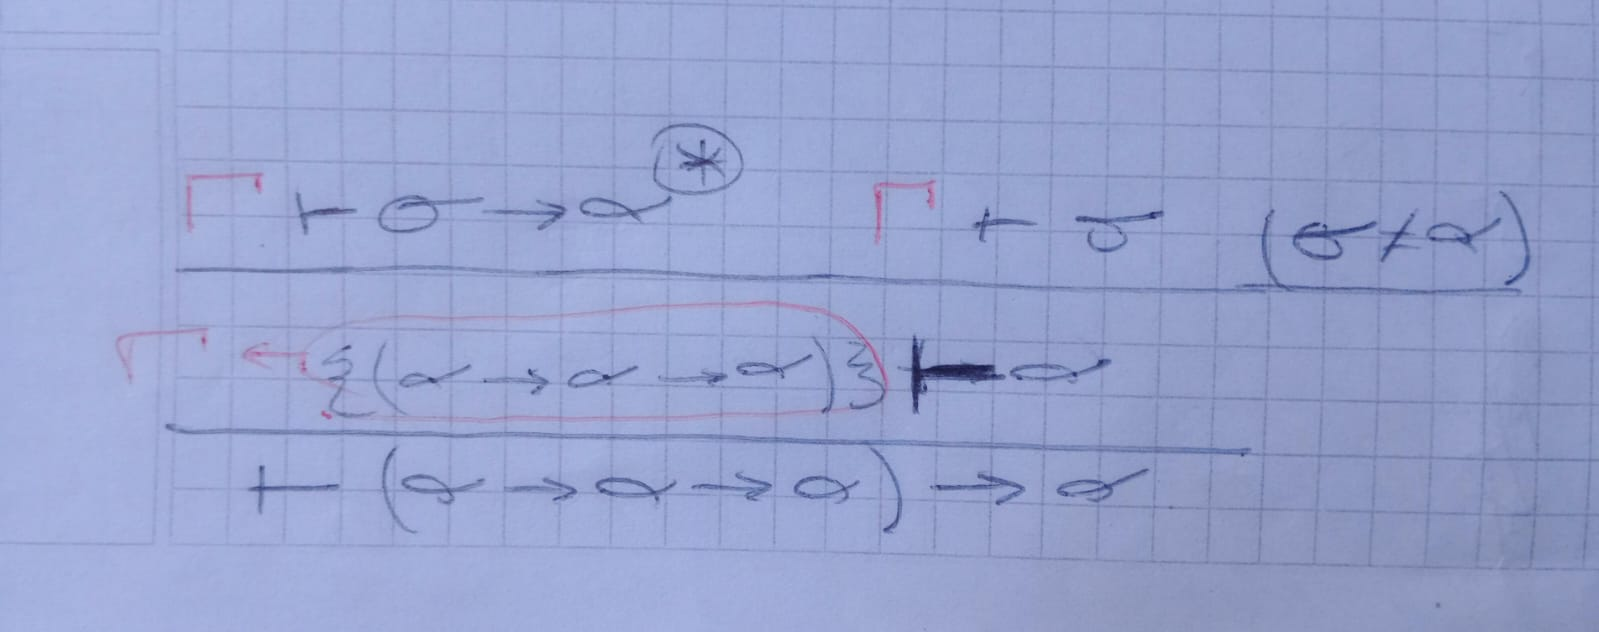
\includegraphics[scale=0.2]{ej2a1.jpeg}
\caption{Supuesto juicio de tipado de $(\alpha \rightarrow \alpha \rightarrow \alpha) \rightarrow \alpha$. El tipo $\sigma$ no puede ser igual a $\alpha$, ya que sino tendríamos un juicio de tipado infinito.}
\label{fig:ej2a1}
\end{figure}

El juicio de tipado $\Gamma \vdash \sigma \rightarrow \alpha$ podría ser una aplicación de dos reglas de tipado posibles: la Abs, o la App. En ambas se alcanza a que es necesario deducir un juicio de tipado que crece o en el tamaño del tipo, o en el tamaño del contexto de tipado. Esto se puede ver en las Figuras~\ref{fig:ej2a2} y~\ref{fig:ej2a3}. Como nunca decrece, el juicio de tipado es infinito, y por lo tanto no es un juicio válido. Por ende, no existe un término cerrado de tipo $(\alpha \rightarrow \alpha \rightarrow \alpha) \rightarrow \alpha$.

\begin{figure}[htbp]
    \centering
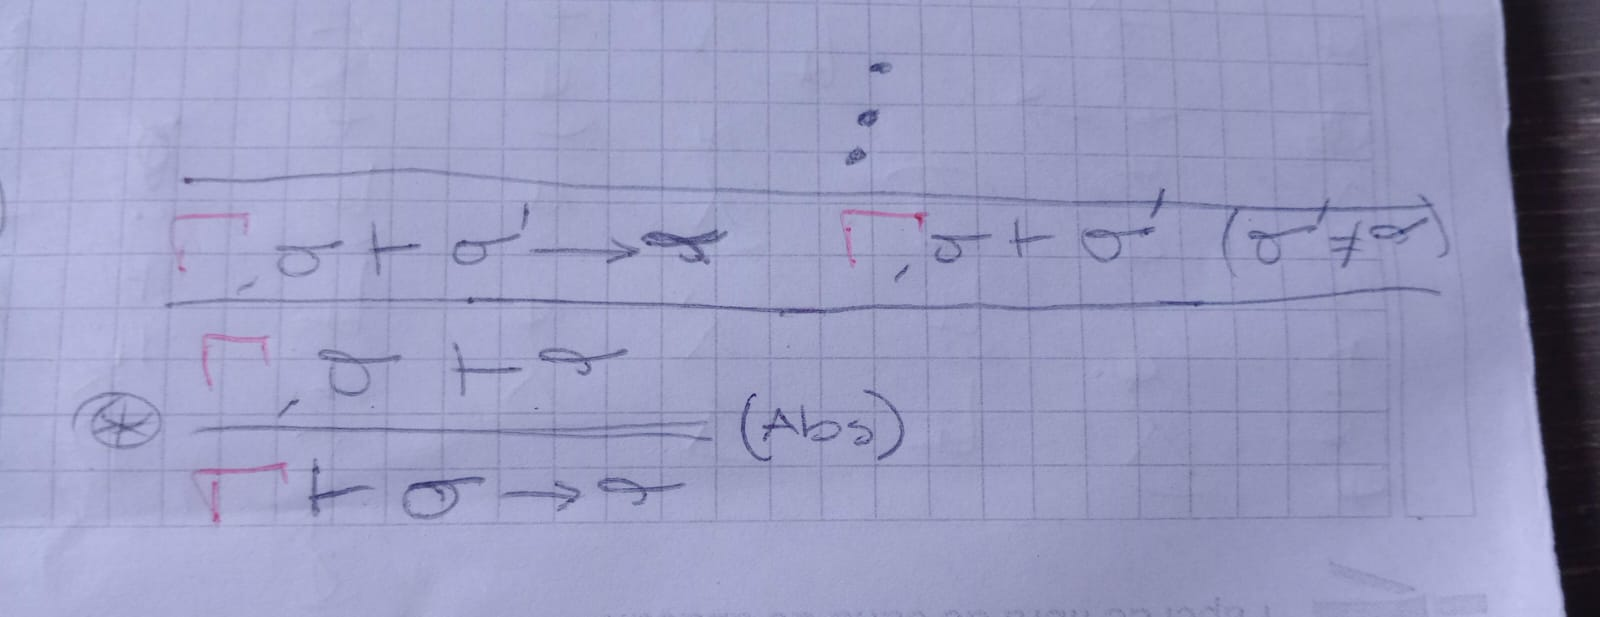
\includegraphics[scale=0.2]{ej2a2.jpeg}
\caption{Continuación del juicio de tipado aplicando la regla Abs. Obligatoriamente se tiene que aplicar la regla App para continuar el juicio de tipado, ya que $\alpha \not\in \Gamma, \sigma$.}
\label{fig:ej2a2}
\end{figure}


\begin{figure}[htbp]
    \centering
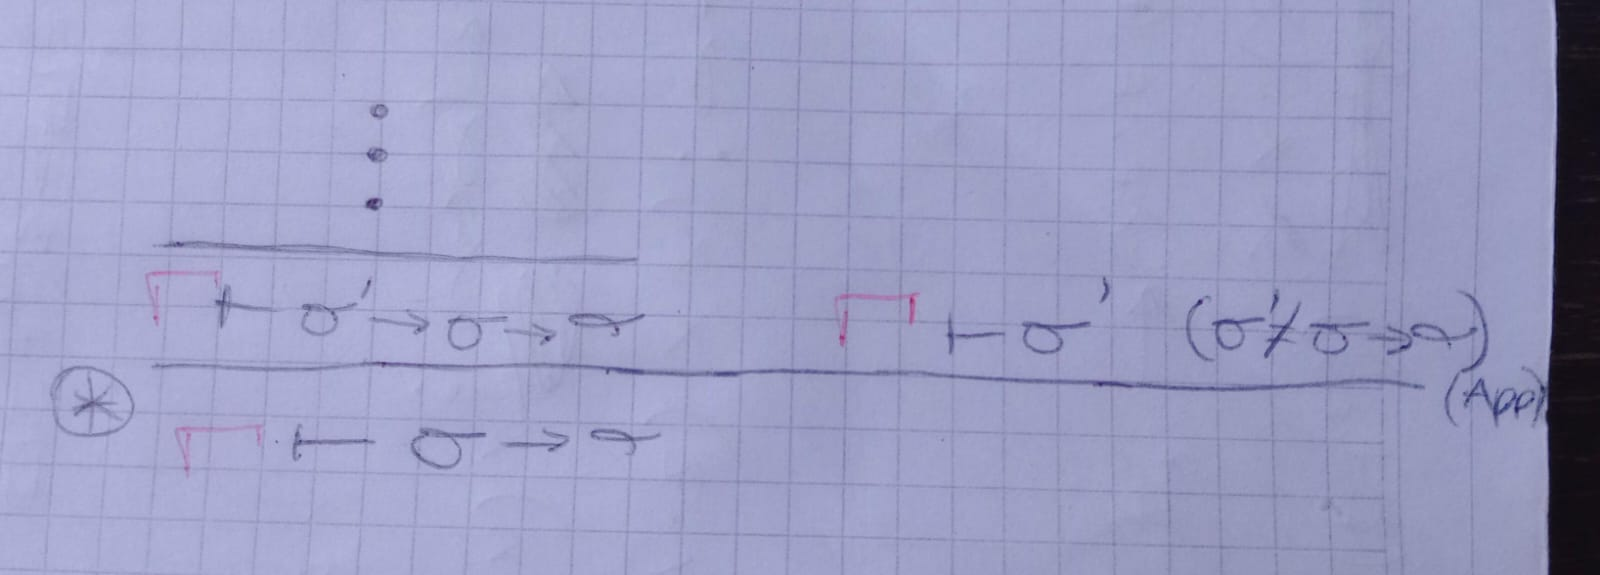
\includegraphics[scale=0.2]{ej2a3.jpeg}
\caption{Continuación del juicio de tipado aplicando la regla App.}
\label{fig:ej2a3}
\end{figure}

\subsection*{b) Existe un término cerrado de tipo $((\alpha \rightarrow \alpha) \rightarrow \alpha) \rightarrow \alpha$.}

\textbf{Verdadero.} El juicio de tipado se puede ver en la Figura~\ref{fig:ej2b}. En particular, el término que satisface el juicio de tipado es $(\lambda f. f\ I)$, donde $I$ es la identidad.

\begin{figure}[htbp]
    \centering
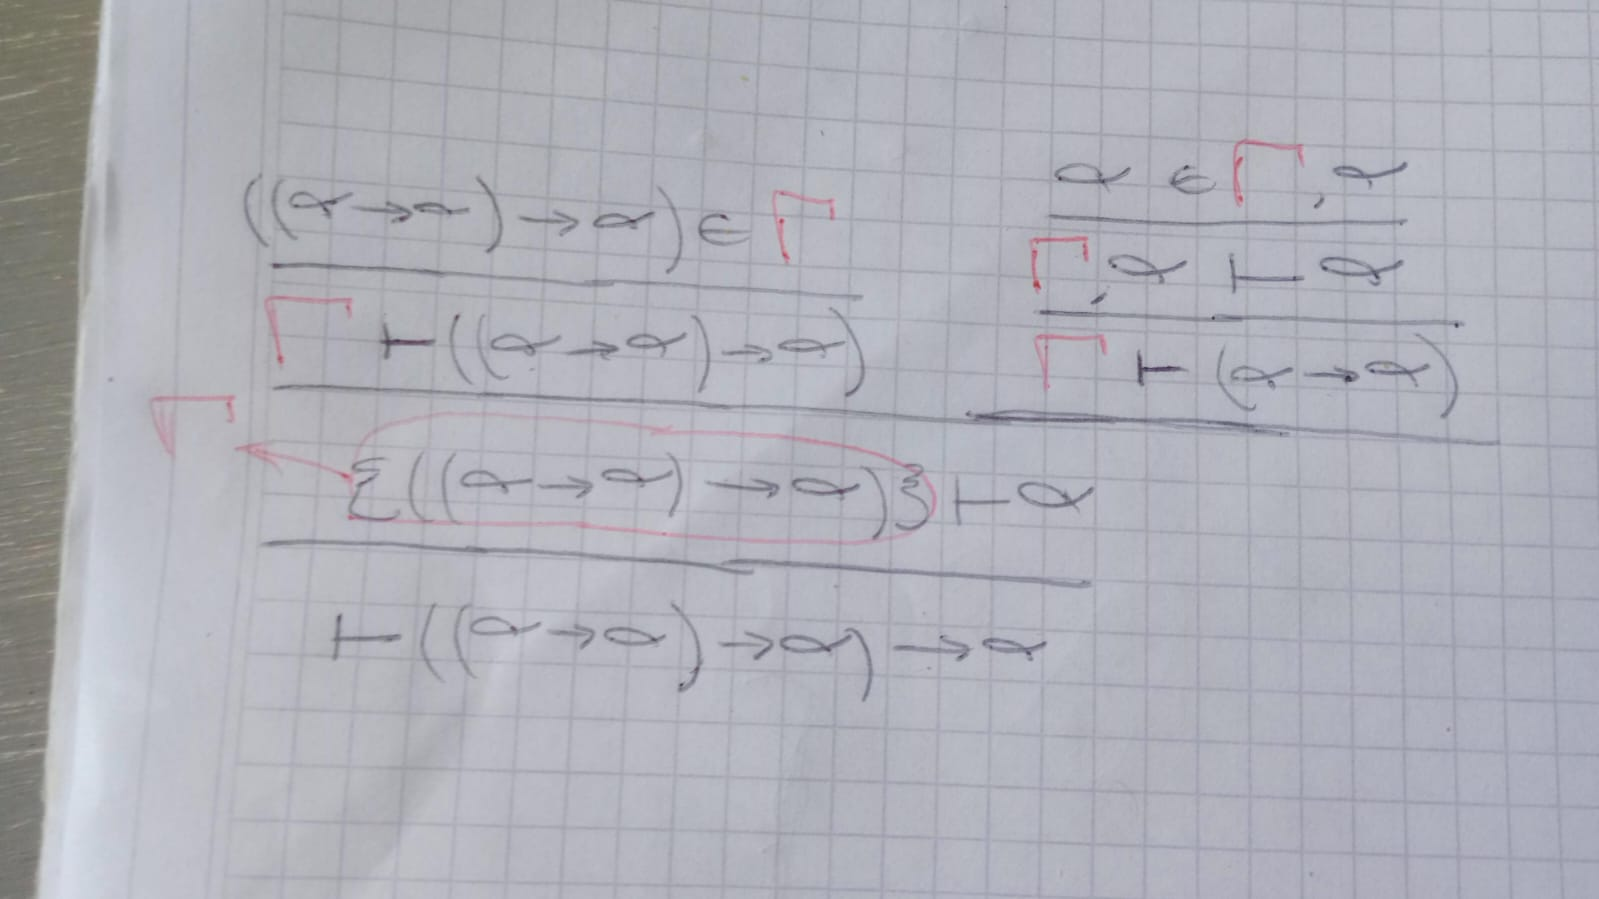
\includegraphics[scale=0.2]{ej2b.jpeg}
\caption{Juicio de tipado de $((\alpha \rightarrow \alpha) \rightarrow \alpha) \rightarrow \alpha$.}
\label{fig:ej2b}
\end{figure}

\section*{Ejercicio 3}

Por lo visto en clase, si un término es tipable en el cálculo-$\lambda$ simplemente tipado, entonces es SN. Veremos entonces que $t_i$ es tipable para todo $i$. Para esto, es suficiente con ver que $t_i$ reduce a un término tipable.

Primero, $t_0 = z$ es tipable con un tipo atómico $a$. Ahora, veremos que $t_i$ tiene también tipo $a$ para todo $i > 0$.

Supongamos que $t_{i-1}$ tiene tipo $a$. Notar que $F$ reduce a $I = (\lambda x.x)$. Reduciendo $t_i$ tenemos entonces que
\begin{align*}
    t_i &= (\lambda f. f (f\ t_{i-1})) F\\
    &\rightarrow_\beta (\lambda f. f (f\ t_{i-1})) I\\
    &\rightarrow_\beta I (I\ t_{i-1})\\
    &\twoheadrightarrow_\beta t_{i-1}.
\end{align*}
Como $t_{i-1}$ es tipable por hipótesis, $t_i$ también lo es, y por lo tanto es SN.
\end{document}